\newtheorem{definition}{Definition}
\newtheorem{example}{Example}

The algorithm's primary objective is to detect reverted sequences within a target DNA sequence, which are characterized by segments that have been inverted and complemented relative to a reference DNA sequence. \\
It uses sample-specific strings as possible anchors of an inverted portion occurring in the target.

\section{Definitions}
In this paragraph will be introduced the definitions that will be used throughout the thesis. \\
The definition of sample-specific string\cite{khorsand_comparative_2021} is as follows:

\begin{definition}[Sample-specific string (SFS)]
A sample-specific string S is a string that occurs in the target DNA string T, does not occur in the reference DNA string R, and for every string S' which is a substring of S, S' occurs in the reference string R. 
\label{thm:sample_specific}
\end{definition} 

Subsequently, it will be necessary to formally define what constitutes an inverted segment of the target $T$ in relation to the reference $R$. The following definitions establish these key concepts:

\begin{definition}[Inversion]
Let $T$ be a target string and $R$ a reference string. A substring $s = T[i,j]$ for $1 \leq i < j \leq |T|$ is a single inversion in the target $T$ with respect to $R$ if $s^{rc}$ occurs as a substring of $R$. If the inversion in $T$ occurs from $i$ to $j$, it is denoted as a triple $(T, i, j)$.
\end{definition}

Next, the concept of substring from $i$ to $j$ is defined, along with the notion of a single inversion:

\begin{definition}[Substring]
Given a string \( S \), the substring \( S[i:j] \) is defined as the sequence of characters in \( S \) that starts at position \( i \) (inclusive) and ends at position \( j \) (exclusive). Formally, \( S[i:j] = s_i s_{i+1} \ldots s_{j-1} \), where \( s_k \) represents the character at position \( k \) in the string \( S \), and \( 0 \leq i < j \leq |S| \).
\end{definition}

\begin{definition}[Single Inversion]
Given a string $S$, another string $S'$ is obtained by a single inversion on $S$ from $i$ to $j$ if $S'$ is derived by reversing and complementing $S[i,j]$, denoted as $S[i,j]^{rc}$.
\end{definition}

Finally, the concept of inversion breakpoint is introduced:

\begin{definition}[Inversion Breakpoint]
Given an inversion $(S', i, j)$ in string $S'$ with respect to string $S$, the indexes $i$ and $j$ are referred to as breakpoints of the inversion if $S[i,j] = S'[i,j]^{rc}$, and no index $i' < i$ or $j' > j$ exists such that $S[i',j'] = S'[i',j']^{rc}$.
\end{definition}

These definitions will be used in the description of the algorithm for solving the Detecting-Inversions problem, described in Chapter 3. In cases involving multiple inversions, the target may result from several disjoint inversions.\\

Since the Knuth-Morris-Pratt algorithm will be introduced in Section 2.4 below as the method used to verify the presence of the middle segment between two sample-specific strings (extracted from the target) within the reference, a few clarifying definitions\footnote{https://proofwiki.org/wiki/Definition:Prefix} are presented here:

\begin{definition}[Proper prefix]
Given a string $S$, a string $T$ is a prefix of $S$ if and only if $S$ can be formed by concatenating $T$ with another string $T'$. If $S = TT'$, $T$ is a proper prefix of $S$ if $T' \neq \varepsilon$, meaning $T'$ is not the empty string.

\label{thm:proprefix}
\end{definition}

\begin{definition}[Proper suffix]
Given a string S, a string T is a suffix of S if and only if S can be formed by concatenating another string T' with T. If $S = TT'$, $T'$ is a proper suffix of $S$ if $T \neq \varepsilon$, meaning $T$ is not the empty string.
\label{thm:prosuffix}
\end{definition}

\section{Biological Background}

\subsection{DNA}

Before addressing the computational part of the project, it is useful to present an overview of its biological background. \\
Deoxyribonucleic acid (DNA) is the molecule that carries genetic information for the development and functioning of an organism\footnote{https://www.genome.gov/genetics-glossary/Deoxyribonucleic-Acid}. Each DNA molecule consists of a long polymer made up of repeating units, the nucleotides, which are composed of a phosphate group, a sugar molecule, specifically 2-deoxyribose, and a nitrogenous base. There are four types of nitrogenous bases found in DNA that define the properties of the nucleotide: adenine (A), thymine (T), guanine (G), and cytosine (C), as shown in Figure \ref{fig:dna}.\\

\begin{figure}[h]

  \centering
    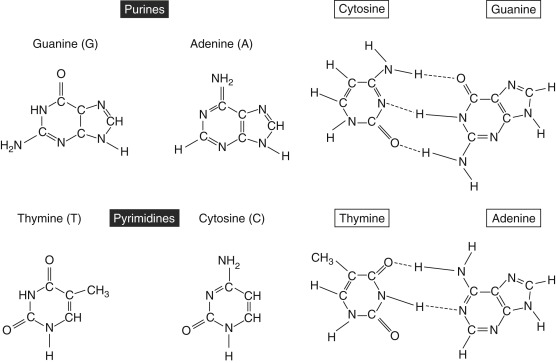
\includegraphics[width=250px]{dna.jpg}

  \caption{DNA nucleotide bases and base pairing.}
  \label{fig:dna}
\end{figure}

In all eukaryotic organisms, DNA exists as a tightly associated pair of two long strands that intertwine, forming the shape of a double helix. The two strands of DNA are stabilized by hydrogen bonds between the nitrogenous bases attached to the two strands \cite{carter_chapter_2022}. Watson-Crick base pairing involves adenines pairing with thymines and guanines pairing with cytosines. Strands of DNA that form matches among base pairs are called complementary strands. \\

\subsection{Double strand breaks}

Double-strand break (DSB) is the primary cytotoxic lesion generated by ionizing radiation, radio-mimetic chemicals such as camptothecin (CPT), mechanical stress on chromosomes, or when the replication machinery encounters a single-strand DNA break or other types of DNA lesions. In addition to this, DSBs can also be produced during physiological processes, such as recombination or meiosis \cite{ting_rad18_2010}.
DSBs are a particularly dangerous form of DNA damage because they can lead to chromosome loss, translocations or truncations. Repair occurs via one of two pathways: non-homologous end-joining (NHEJ), in which broken DNA ends are directly ligated; or homologous recombination (HR), in which a homologous chromosome is used as a template in a replicative repair process. 

\subsection{DNA recombination and formation of inversions}

Genetic recombination is a fundamental cellular process that has a role in the generation of genetic diversity, in the repair of damaged DNA, in the homologous alignment of chromosomes required for successful completion of meiotic cell division, and in the generation of genomic alterations that lead to changes in gene expression. Classical homologous recombination is a type of genetic recombination in which nucleotide sequences are exchanged between two similar or identical molecules of DNA, as shown in Figure \ref{fig:hr}. During the formation of egg and sperm cells (meiosis), paired chromosomes from the male and female parents align so that similar DNA sequences can cross over, or be exchanged, from one chromosome to the other. This exchange of DNA is an important source of the genomic variation seen among offspring\footnote{https://www.genome.gov/genetics-glossary/homologous-recombination}.
This allelic homologous recombination repairs double-stranded breaks (DSBs) in chromosomes by using the allele on the sister chromatid as a template. This mechanism is highly faithful because the allelic region of the sister chromatid is a nearly exact copy of the DNA lost in the DSB \cite{parks_detecting_2015}. 

\begin{figure}[h]

  \centering
    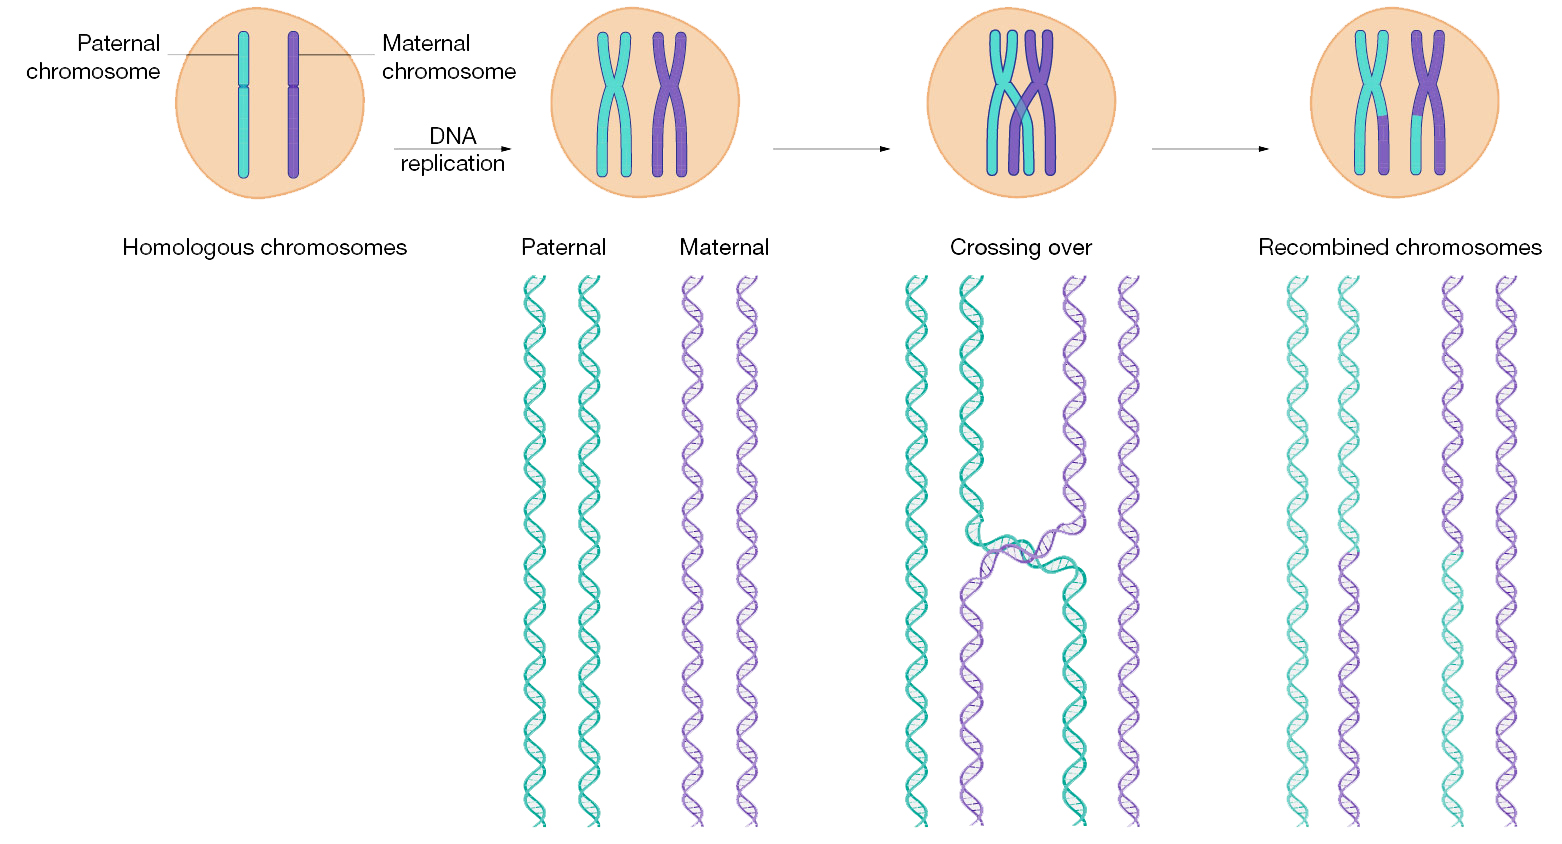
\includegraphics[width=375px]{hr.jpg}

  \caption{Homologous recombination between maternal and paternal chromosomes.}
  \label{fig:hr}
\end{figure}

However, a similar recombination process can also occur between repetitive DNA sequences that are similar but located in different (non-allelic) regions of the genome. This process is called non-allelic homologous recombination (NAHR). \\
It occurs between Low Copy Repeats (LCRs), also known as Segmental Duplications, that are DNA blocks of 10 to 400 kb in size with over
97\% identity between sequences \cite{burssed_mechanisms_2022}. NAHR can occur after a DSB during meiosis or mitosis when non-allelic copies of LCRs erroneously align due to their high level of sequence identity. This misalignment causes an unequal crossing over event generating genomic rearrangement in the daughter cells. 

\begin{figure}[h]

  \centering
    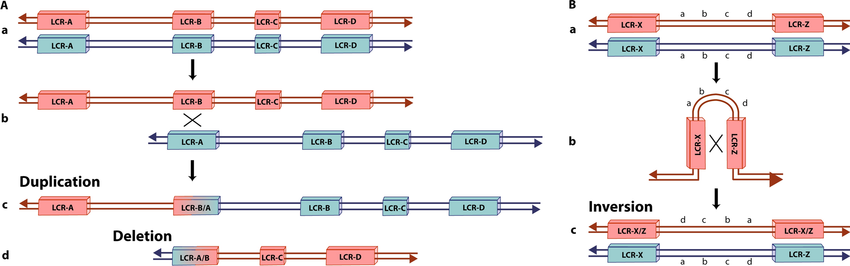
\includegraphics[width=400px]{nahr.png}

  \caption{Non-Allelic Homologous Recombination (NAHR) mechanism. A. NAHR leading to the formation of duplication and deletion: (a) Normal chromosome pairing and alignment of Low Copy Repeats (LCRs) in the same orientation. (b) A misalignment between LCRs due to their high level of sequence identity leads to an unequal crossing over event that can generate (c) a duplication and (d) a deletion. B NAHR leading to the formation of inversions: (a) Normal chromosome pairing and alignment of Low Copy Repeats (LCRs). LCR-X and LCR-Z present similar DNA sequences but in opposite orientations. (b) A misalignment between LCRs due to their high level of sequence identity leads to an unequal crossing over event that can generate (c) an inversion}
  \label{fig:nahr}
\end{figure}

Through NAHR, regions located between segmental duplications or highly identical repeat sequences may be deleted, duplicated or inverted. Inversions can be formed by this process if the duplicated sequences are in inverted orientation with respect to each other, as Figure \ref{fig:nahr}B shows. Therefore, NAHR is considered the primary mechanism by which large (tens of kilobases) inversions are formed \cite{feuk_inversion_2010}. 

\section{Inversion in human disorders}

Many inversions traditionally detected in human karyotypes do not appear to have any phenotypic effects of clinical significance. This is the case of pericentric inversions (the inverted sequence includes the centromere) in chromosomes 1, 2, 3, 5, 9, 10 and 16. These mainly invert heterochromatic sequences and are frequently observed in cytogenetic analysis \cite{puig_human_2015}. However, not all inversions are harmless, and several diseases have been found to be occasionally caused by inversions, mostly due to direct disruption of one gene or alteration of its gene expression. These inversions appear de novo in patients or are inherited mutations restricted to a given family. \\
Since inversions are relatively rare events, and it is unlikely to have multiple patients with the same inversion, it is often problematic to assess whether the inversion present in the patient is actually associated with the phenotype. The exception is when the inversion breakpoint falls within or near a gene that has previously been associated with a disorder through other types of mutations. For recurrent inversions, the association between phenotype and genotype is more obvious, and a number of such loci have been described. One of the best-characterized disease-triggering recurrent inversions is linked to hemophilia A, an X-linked disorder caused by mutations in the factor VIII gene. A recurrent inversion has been found in approximately 43\% of patients.
Molecular characterization of the breakpoints indicates that the inversion is a result of intra-chromosomal homologous recombination, originating almost exclusively in male germ cells. This recurrent inversion spans approximately 400 kb and is mediated by two inverted segmental duplications, one of which is located in intron 22 of the factor VIII gene, with two other copies being located approximately 400 kb telomeric to the gene. Other examples where recurrent inversions have been shown to lead to a disease phenotype are the disruption of the idunorate 2-sulphatase gene in mucopolysaccharidosis type II (Hunter syndrome), and disruption of the emerin gene in Emery-Dreifuss muscular dystrophy \cite{feuk_inversion_2010}. \\
In addition to this, it was found that the presence of micro-inversions, defined as inversion in DNA shorter than 100 bp, can be linked to cancer, as shown by a study conducted in 2018 \cite{qu_micro-inversions_2018}. This study analyzed the distribution of micro-inversions among 24 chromosomes in four types of cancer (hepatocellular, lung, pancreatic and bladder), and found that the average count of micro-inversions per individual in the normal samples was lower than that of any type of cancer, showing that there is a high chance that micro-inversions may be associated with cancer development (see Figure \ref{fig:cancer}).

\begin{figure}[h]

  \centering
    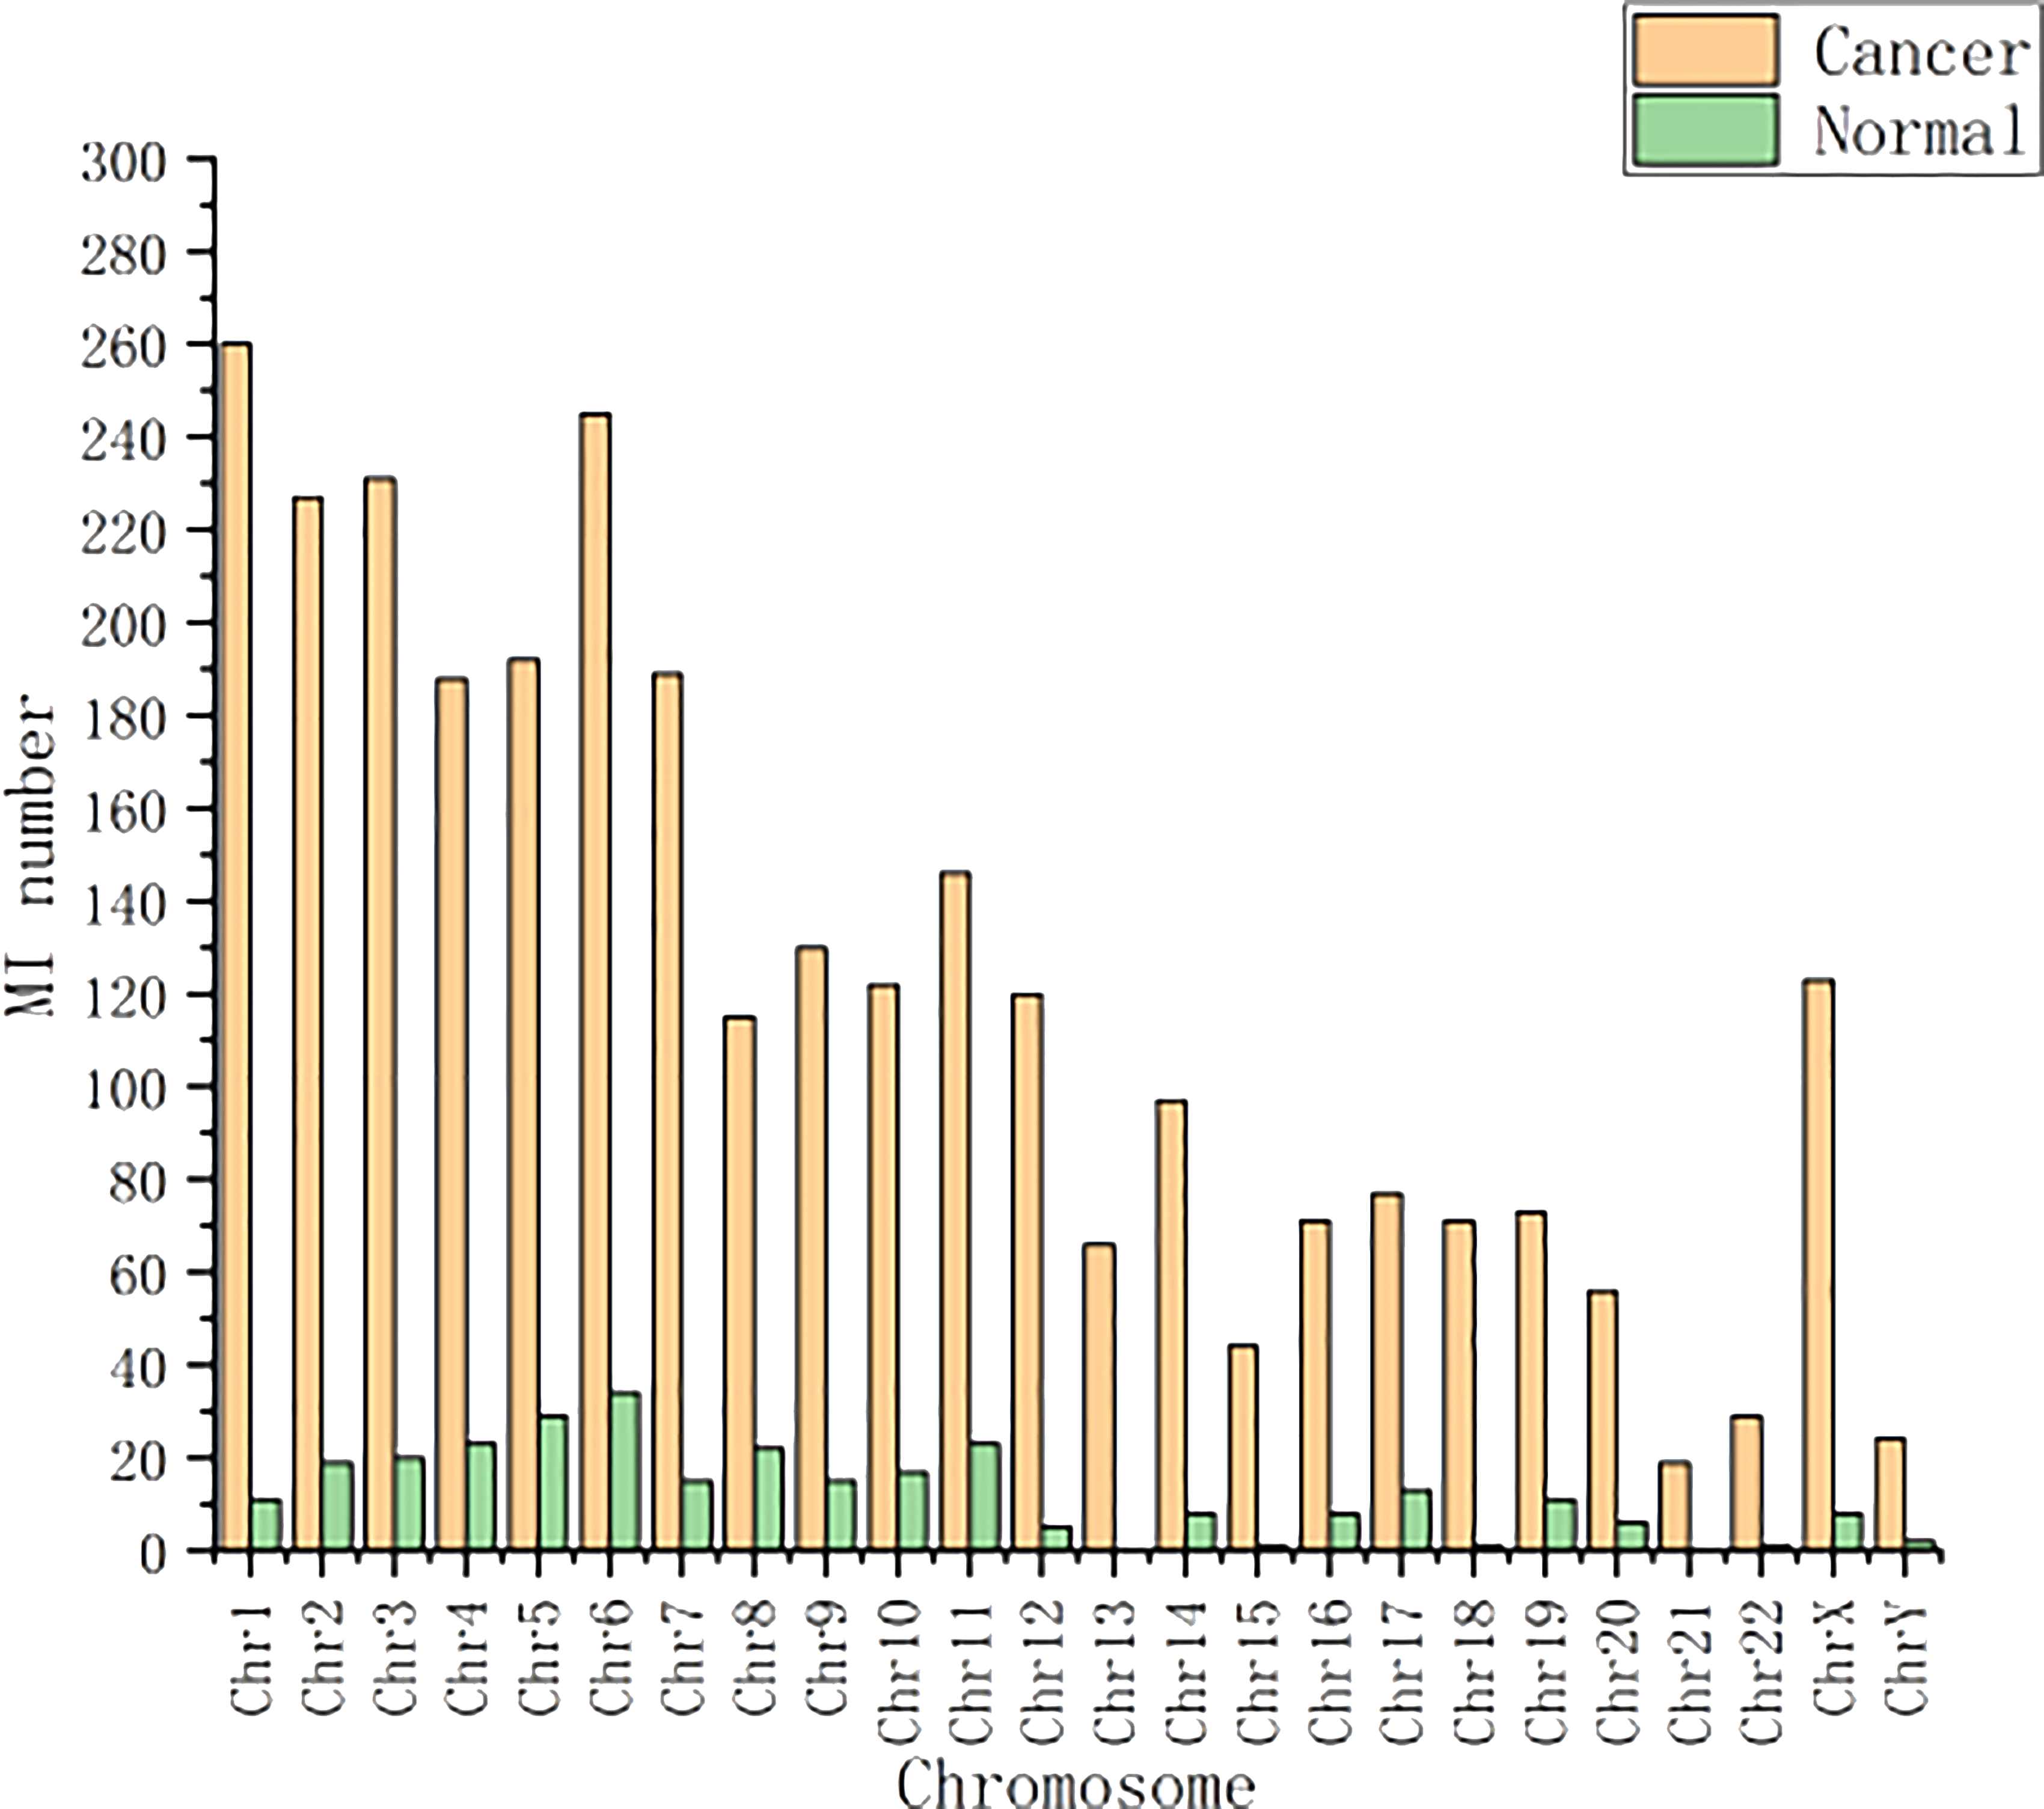
\includegraphics[width=250px]{cancer.png}

  \caption{Micro-inversion (MI) distribution among 24 chromosomes.  Average count of MIs per individual among the four types of cancer.}
  \label{fig:cancer}
\end{figure}
\newpage
\section{Knuth-Morris-Pratt Algorithm}

Knuth-Morris-Pratt \cite{knuth_fast_1977} (KMP) is the algorithm that will be used in this project to detect the position of inverted segments within the reference. It can be seen as an evolution of the naïve string-matching algorithm. In fact, given a text \textit{T} having length \textit{n} and a pattern \textit{P}, the naïve algorithm, for each possible starting position \textit{i}, where 0 \leq \textit{i} \leq \textit{n} - \( m \), compares the substring starting at position \textit{i} in the text with the pattern. If a mismatch is found, it moves to the next position. If all the characters match, it returns the occurrence of the pattern at index \textit{i}. \\
The idea behind the Knuth-Morris-Pratt algorithm is that, in case of mismatch, it is possible to perform a shift greater than 1, in order to avoid unnecessary comparisons. 

\subsection{LPS array}
KMP preprocesses the pattern by building an auxiliary array, the Longest Prefix Suffix (LPS) array. For each index \( i \) of the pattern \( P \), \( LPS[i] \) contains the length of the longest proper prefix of the substring \( P[:i] \) which is also a suffix of said substring. This array is the key to the algorithm’s efficiency. It helps in skipping characters that will certainly match, thus reducing the number of comparisons needed and ultimately speeding up the search process.  \\
The process of building the LPS array can be described as follows:

\begin{itemize}
\item Initialization: an array \( LPS[] \), of size equal to the length of the pattern is initialized with zeros. \( LPS[0] \) is set to 0 because there is no proper prefix for a single character. Two pointers are also initialized: \( i \), which iterates through the pattern, is set to 1, and \( j \), which will track the length of the previous longest proper prefix suffix, is set to 0.
\item Iteration over the pattern: each character at index \( i \) in the pattern is compared with the character at index \( j \) in the text. If \( P[i] == P[j] \), the current character in the pattern extends the longest proper prefix that is also a suffix, so both indexes \( i \) and \( j \) are incremented and \( LPS[i] = j\). Otherwise, if \( P[i] != P[j] \), the previously computed \( LPS[j-1] \) is checked to determine the next smaller prefix that could still match. If \( j == 0 \), there is no valid prefix to fall back to, so \( LPS[i] \) is set to 0 and \( i \) is incremented in order to move to the next character. 
\end{itemize}

The process continues until \( i\) reaches the length of the pattern.

\begin{figure}[h]

  \centering
    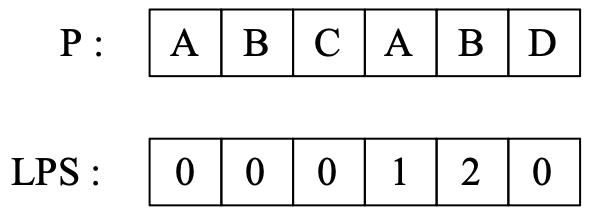
\includegraphics[width=250px]{lps.png}

  \caption{For the pattern \( P \) displayed in the figure, for the first three positions, \( LPS[i] \) equals to 0 because there is no proper prefix for "A", "AB" or "ABC" which is also a suffix. Moving on, \( LPS[3] \) is 1 because the proper prefix "A" of "ABCA" is also a suffix, \( LPS[4] \) is 2 because the proper prefix "AB" of "ABCAB" is also a suffix. For the last position, \( LPS[5] \) is, again, 0, since no proper prefix of "ABCABD" is also a suffix.}
  \label{fig:lps}
\end{figure}

\subsection{Pattern matching}

The KMP algorithm iterates through the text \( T \) and through the pattern \( P \), using two separate pointers. When a character in the reference matches a character in the pattern, both pointers are incremented to continue the comparison. 
When a mismatch is found at position  \( j \) in the reference and \( i \) characters of the pattern have already been matched, instead of restarting from the beginning of the pattern as it happens in the naïve algorithm, KMP consults \( LPS[i-1] \) in order to determine how many characters of the pattern can be skipped. Thus, the KMP algorithm performs pattern matching in $\mathcal{O}(n + m)$ time, where \( n \) is the length of the reference and \( m \) is the length of the pattern.

\begin{figure}[h]

  \centering
    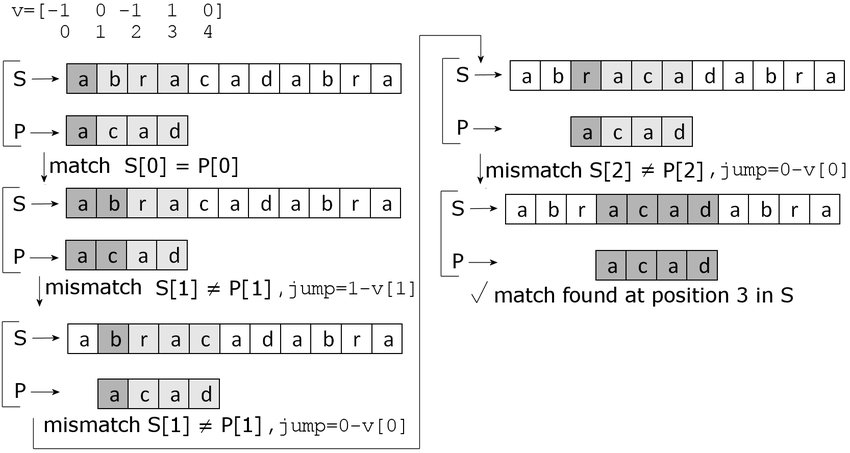
\includegraphics[width=300px]{kmp.jpeg}
  \label{fig:kmp}
\end{figure}

Among other solutions, like the suffix array or the Boyer-Moore algorithm, the KMP algorithm was chosen for this project because it is more suitable in contexts with a very limited alphabet, such as DNA ({A, C, T, G}). Additionally, KMP performs well even when the length of the reference is large, unlike, for example, the suffix array method, which which can become less efficient in such cases due to its preprocessing requirements. This makes KMP the optimal choice for detecting inversions from long reads in the reference. 

\section{DNA sequencing}

In bioinformatics, DNA sequencing is the process of determining the sequence of nucleotides (As, Ts, Cs, and Gs) in a strand of DNA. A read is defined as a raw sequence generated by a sequencing machine\footnote{https://samtools.github.io/hts-specs/}. A read may consist of multiple segments. For sequencing data, reads are indexed in the order in which they are sequenced. Most next-generation sequencing technologies fragment the genome prior to sequencing, and each sequenced fragment produces a read. The length of the read and how many are produced will depend on fragment size and the type of technology used. As the fragments of DNA usually overlap, the reads can be pieced back together to reconstruct the genome. The length of the read is the number of bases that are read at one time, hence the number of letters that will appear in each read. In general, they can be divided into:

\begin{itemize}
\item \textbf{Short reads: } have lengths usually ranging from 50 to 300 base pairs. They are effective for applications aimed at counting the abundance of specific sequences, identifying variants within otherwise well-conserved sequences, or for profiling the expression of particular transcripts. Short-read sequencing is the best way to obtain high-depth, high-quality data at the lowest cost per base. On the other hand, short reads fail to generate a sufficient overlap between the DNA fragments. Overall, this means that it can be challenging to use them for sequencing highly complex, repetitive libraries, like the human genome. The dominant technologies in this field are Illumina’s platform and Thermo Fisher Scientific’s Ion Proton. However, multiple new sequencing technologies have surfacedin 2022, and have now been introduced to the market, helping to drive short-read sequencing costs even lower. These include instruments from Element Biosciences, Ultima Genomics, MGI, Singular Genomics and the PacBio acquired technology, Omniome\footnote{https://frontlinegenomics.com/long-read-sequencing-vs-short-read-sequencing/}. 
\item \textbf{Long reads: } have lengths usually ranging from 5000 to 50000 base pairs \cite{lee_error_2014}. They allow to identify complex SVs such as large insertions/deletions, inversions, repeats, duplications, and translocations. Long read NGS instruments have been on the market for the past decade but the lower yield, higher error rate, and higher costs of the instruments, have kept them from being more widely adopted. An additional downside is that the accuracy per read can be much lower than that of short-read sequencing. In the last decade, PacBio and Oxford Nanopore Technologies (ONT) have both been working to make long-read sequencing more accessible. Specifically, PacBio has improved the chemistry on their Sequel II instruments, enabling “HiFi sequencing” via circular consensus, which allows for sequencing of up to 15-20 kb pieces of DNA with error rate that are closer to short read sequencing.

\end{itemize}

Sequencing data are the main input of several bioinformatics algorithms. The algorithm described in this work uses long read sequencing data. Indeed, due to their length, they are suited to detect enough long inversions. 

\section{FASTA format}

FASTA is a text-based format used in bioinformatics to represent DNA sequences, in which base pairs are represented using a single-letter code from the alphabet \(\Sigma = \{A, C, G, T\}\),  where each letter corresponds to the initial of one of the four nitrous bases that make up the DNA. The format also allows for sequence names and comments to precede the sequences. As detailed in Chapter 4 below, FASTA will be used in this project to represent both the reference sequence and the target, which is a long read of the reference. A FASTA sequence begins with a single-line identifier description, followed by lines of DNA sequence data. The identifier description line is distinguished from the sequence data by a greater-than ('\( \textgreater \)') symbol in the first column. The word following the "\( \textgreater \)" symbol is the identifier of the sequence, and the rest of the line is an optional description separated from the identifier by a white space or tab. The sequence data starts on the next line following the text line and ends at the appearance of another line starting with a "\( \textgreater \)", which signals the start of another sequence. The extension of this format is usually \texttt{.fa}. 

\begin{example}
  This is an example of a portion of a FASTA file that contains two nucleotide sequences:
\begin{verbatim}
>NC_045512.2 
ATTAAAGGTTTATACCTTCCCAGGTAACAAACCAACCAACTTTCGATCTCTTGTAGATCT
GTTCTCTAAACGAACTTTAAAATCTGTGTGGCTGTCACTCGGCTGCATGCTTAGTGCACT
>OL700521.1 
GTTCTCTAAACGAACTTTAAAATCTGTGTGGCTGTCACTCGGCTGCATGCTTAGTGCACT
CACGCAGTATAATTAATAACTAATTACTGTCGTTGACAGGACACGAGTAACTCGTCTATC
\end{verbatim}
\end{example}



